\section{Développement d'un simulateur de données brutes}
\label{sec:simulateur}
Après avoir fait le choix de nos algorithmes de traitement, il faut les valider dans nos conditions expérimentales. Il était souhaité d'utiliser des données expérimentales assez rapidement, notamment car le module RF avait été présenté comme clé en main et prêt à être utilisé. Comme nous avons rencontré plusieurs problématiques concernant ce module, la question de la simulation et de la génération de données brutes s'est posée.

Ce simulateur a été réalisée en plusieurs étapes. Tout d'abord nous nous sommes basés sur les travaux de Mathworks \cite{mathworks_stripmap_sar} et les avons adaptés aux paramètres expérimentaux inhérents à la plateforme radar ST200 de RFBeam avec le transceiver K-MC4. Cependant ce simulateur ne réplique pas tout à fait le fonctionnement du transceiver choisi. En effet, ce dernier simule l'émission et la réception d'impulsions radar alors que le module RF récupère uniquement la fréquence de battement en FMCW. De plus, le premier simulateur étant conçu pour un radar pulsé, son adaptation nécessitait une fréquence d'échantillonnage supérieur à deux fois notre bande ($\approx400 MHz$). Or notre carte échantillonne à $250kHz/s$, il était donc nécessaire d'adapter la logique de simulation pour pouvoir valider nos algorithmes.

Ainsi, les travaux d'adaptation effectués sur la version de Mathworks nous ont permis de recréer un simulateur qui cette fois-ci ne représente que la fréquence de battement. Comme expliqué dans la partie \ref{subsec:formes_ondes}, cette fréquence de battement permet de déterminer la distance radiale d'une cible ce qui nous permettra de reconstruire notre image avec l'algorithme choisi. 

\subsection{Choix d'architecture}\label{subsec:choix_archi_simu}
Cette partie se concentrera sur la justification et l'explication des choix techniques effectués durant le développement du simulateur. Tout abord nous aborderons le choix du langage de programmation puis les différentes modélisations utilisées.

\subsubsection{Langage de programmation utilisé}\label{subsubsec:choix_langage_simu}
En tenant compte des compétences des membres de l'équipe traitement et du contexte, deux langages sortent du lot ; MATLAB et Python. En effet, ils sont utilisés pour de la programmation scientifique, sont relativement performant et accessible. Or, les membres de l'équipe sont plus à l'aise avec Python, nous avons donc essayé de réaliser le portage du code MATLAB vers Python. Cependant, les différences de nomenclatures, d'interprétation, de représentations matricielles et autres le rendent complexe et chronophage. Le langage de programmation retenu est donc MATLAB.

Ensuite, nous souhaitions mettre en place la parallélisation des calculs mais pour cela il fallait avoir accès à une machine avec GPU/TPU. Il est possible d'installer MATLAB sur un notebook Google Colab mais cela est lent et fastidieux puisque l'installation prend cinq minutes et n'est pas persistante. De plus, l'exécution de code MATLAB se fait via un module Python et l'hébergement d'une version WEB, qui n'est pas maîtrisée et qui a donc potentiellement quelques effets de bord. Après plusieurs tests, les simulations sont assez courtes avec nos ordinateurs personnels (quelques secondes à minutes), nous resterons donc sur nos ordinateurs personnels pour la suite du développement. 

\subsubsection{Explication détaillée du simulateur}\label{subsubsec:explication_simu}

\paragraph{Choix de l'approche de simulation}
Comme introduit plus tôt, il existe plusieurs façon de réaliser un simulateur. Les deux approches les plus pertinentes dans notre cas sont :
\begin{itemize}
    \item la simulation de l'émission et la simulation des réflexions sur les cibles et le sol,
    \item la simulation de la sortie de la carte d'acquisition.
\end{itemize}

La première méthode possède plusieurs avantages, les plus importants étant la maîtrise de la modélisation de la propagation. En effet, en simulant cette dernière, il est possible de l'ajuster pour s'adapter au mieux au contexte défini. Il est aisé d'ajouter des multi-trajets et le bruit est plus facile à modéliser de manière cohérente. Cette méthode est également plus réaliste en terme de fonctionnement. 

Cependant, elle comporte également quelques désavantages. Tout d'abord, notre plateforme utilisera la forme d'onde FMCW triangulaire avec une bande d'environ $180~MHz$. Cette bande et méthode de simulation impliquent une fréquence d'échantillonnage minimale d'environ $360~MHz$. Or notre carte peut échantillonner avec une fréquence maximale de $250~kHz$ partagée pour chaque antenne et voie (I et Q). Pour cela, la carte utilise un mélangeur permettant d'isoler la fréquence de battement. Bien qu'il serait possible de mettre en place le même mécanisme dans notre simulateur, ce n'est pas pertinent puisque nous devrions simuler tous les composants alors qu'il est possible de simuler directement la fréquence de battement. Cette simplification nous place directement dans le cas où nous simulons uniquement la sortie de la carte d'acquisition. 

Il existe plusieurs avantages à cette méthode, le premier est le faible coût de calcul qui permet de simuler une scène complexe en quelques secondes. Aussi, la simulation étant plus proche des conditions expérimentales, les algorithmes de traitement y seront mieux adaptés.

Maintenant que la logique de simulation est établie, nous pouvons détailler la réalisation et les différents choix effectués. 

\paragraph{Choix des modélisations de simulation}

\subparagraph{Modélisation géométrique de l'antenne}

Le transceiver utilisé par la plateforme est le K-MC4, ce dernier est composé d'une antenne d'émission et de deux antennes de réception. Il est possible de l'utiliser avec l'une des deux antennes de réception désactivée, cependant cela implique une puissance reçue plus faible. Ainsi, pour optimiser au mieux notre signal reçu simulé, nous avons fait le choix de modéliser la réception avec les deux antennes. Il est important de noter que ces deux antennes ne sont pas co-localisées et sont espacées de quelques millimètres. En considérant notre fréquence d'émission, $24~GHz,~ \lambda = 12.5~mm$, nous remarquons que cette distance n'est pas négligeable et doit être prise en compte durant la réalisation du simulateur. 

La structure de l'antenne est maintenant établie, nous pouvons donc aborder la modélisation de son gain. Ce simulateur ayant pour unique objectif de valider la formation d'image et la correction d'erreur, il n'est pas nécessaire de mettre en place une modélisation complexe du gain. En effet, le modèle retenu est une approximation standard du lobe principal. La fidélité du lobe principal est plutôt bonne mais cela ne prends pas du tout en compte la présence de lobes secondaires ou de fuites en arrières comme l'illustre la figure \ref{fig:visu_gain_approx_et_reel}.

\FloatBarrier
\begin{figure}[hbt!]
    \centering
    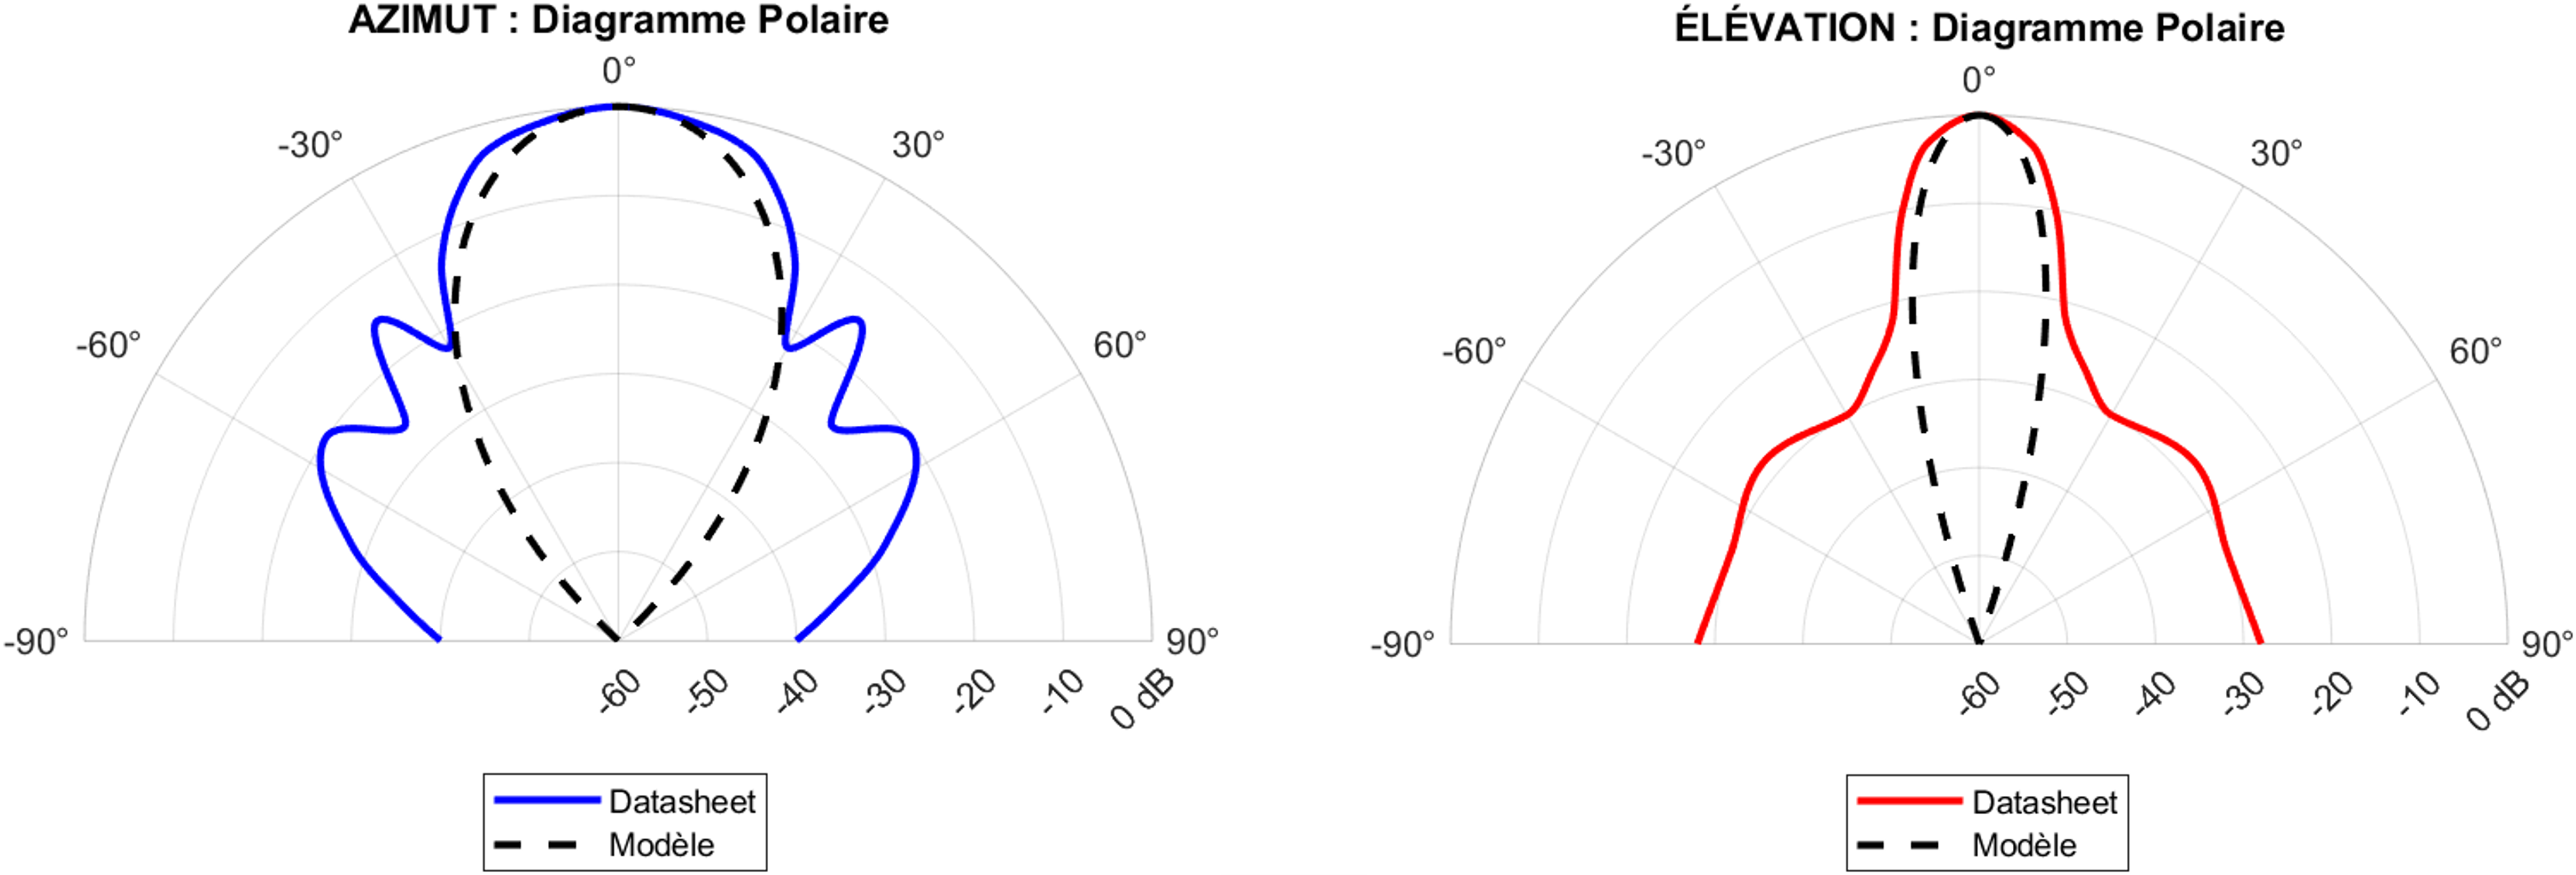
\includegraphics[width=0.8\linewidth]{src/rapport_complet/img/visu_approx_diagramme_antenne_vs_reel.png}
    \caption{Visualisation de l'approximation du gain avec les valeurs mesurées}
    \label{fig:visu_gain_approx_et_reel}
\end{figure}
\FloatBarrier

Visuellement on remarque que l'erreur peut être importante mais il reste important de la quantifier. Pour cela nous utiliserons deux métriques : la RMSE\footnote{Root Mean Square Error/Erreur quadratique moyenne} et la MAE\footnote{Mean Absolute Error/Erreur moyenne absolue}. Utiliser ces deux métriques nous permet de savoir si l'erreur est à peu près constante sur la zone considérée ou non. En effet, la RMSE pénalise les grand écarts à la différence de la MAE, donc un écart significatif entre les deux moyennes impliquent une variance élevée et donc une erreur non constante. 

Après calcul, nous retrouvons ce que nous avions visuellement remarqué : une erreur très importante entre la modélisation simplifiée choisie et les valeurs mesurées (Azimut MAE $53~dB$, RMSE $76~dB$ ; élévation MAE $187~dB$, RMSE $220~dB$. Cependant, le lobe principal est la zone d'intérêt et lorsque le calcul d'erreur y est concentrée, les moyennes sont beaucoup plus faibles :
\begin{itemize}
    \item MAE Azimut ($\pm~15~\degree$) : $0.93~dB$,
    \item RMSE Azimut ($\pm~15~\degree$) : $1.33~dB$,
    \item MAE Élévation ($\pm~6~\degree$) : $0.96~dB$,
    \item RMSE Élévation ($\pm~6~\degree$) : $1.33~dB$.
\end{itemize}
En considérant les différentes problématiques rencontrées sur la carte pour l'adapter en radar imageur et l'objectif du simulateur, une erreur de $\approx1~dB$ dans le lobe principal est tout à fait raisonnable. 

Cependant, l'absence de considération des lobes secondaires et de lobe arrière  met en place un environnement de test parfait qui ne modélise pas le clutter, les fantômes apportés par les réflexions des lobes secondaires et arrières.

\subparagraph{Modélisation du déplacement de la plateforme}
Une fois la géométrie de la carte définie, il faut s'atteler à la modélisation de son déplacement. Nous rappelons que le contexte du SAR demande un déplacement rectiligne suivant l'axe azimut/cross-range (détaillé dans la partie \ref{sec:principes_sar}). Il est alors possible de modéliser le mouvement de deux manières, soit de manière continue soit en utilisant l'approximation Stop\&Go. La première méthode consiste à prendre en compte le déplacement de la plateforme pendant que la pulse est émise, la deuxième considère que la plateforme est immobile pendant l'émission et se déplace instantanément à la position suivante une fois l'émission effectuée. Nous remarquons alors que la première méthode est plus réaliste mais implique une complexité algorithmique plus importante, notamment via le calcul de l'effet Doppler intra-pulse. 

Pour savoir quelle méthode est la plus adaptée à nos besoins, il faut calculer l'erreur induite par l'approximation Stop\&Go. Le VCO de notre transceiver n'est pas de très bonne facture, ce qui implique que nous devons émettre des rampes plutôt longue (quelques microsecondes). Pour simplifier nos calculs, nous considérerons une impulsion de $10~ms$. Il faut maintenant définir la vitesse à laquelle notre plateforme va se déplacer. Comme nous utilisons un bras robot pour nos tests, nous déplacerons la plateforme avec une vitesse faible pour éviter les erreurs de positions dues aux roulis et tangages. La vitesse retenue est de $0.05~m.s^{-1}$. La vitesse de déplacement et la durée d'impulsion retenues nous donne une erreur de position de $0.5~mm$. Cette erreur est bien en deçà de la condition limite nécessaire à la formation d'image SAR, qui est pour rappel $\lambda/8$. Nous pouvons donc utiliser l'approximation Stop\&Go dans notre simulateur.

Cela conclut la mise en place du mouvement idéal de notre drone. Or, en situation réelle, il ne sera pas parfait, il faut donc mettre en place la modélisation des erreurs de trajectoires, notamment des erreurs de roulis, tangages et lacets. 

\subparagraph{Modélisation des erreurs d'attitude}\label{subpar:erreurs_attitude}

Pour étudier la robustesse de nos algorithmes façe aux erreurs d'attitudes du porteur (le type d'erreur de trajectoire le plus impactant dans le cadre de drones), on se propose de modéliser ces erreurs dans notre chaîne de formation d'image. \\ 
On cherche ici un outil qui nous permet de modéliser un vecteur aléatoire avec une autocorélation non nulle sur un efenêtre de temps donnée ce qui permet de modéliser le fait qu'une erreur à un instant dépend de l'erreur à un ensemble d'instants précédents. Cette modélisation n'étant pas possible avec un bruit blanc. On se propose donc d'utiliser un processus de Gauss Markov. \\
Ce processus au premier ordre est régi par l'équation différentielle stochastique suivante :
\begin{equation}
    \dot{x}(t) = -\frac{1}{\tau} x(t) + w(t)
\end{equation}
où $\tau$ représente la constante de temps de corrélation et $w(t)$ est un bruit blanc gaussien de moyenne nulle.\\
L'intérêt de ce processus réside dans ses propriétés statistiques, notamment sa fonction d'autocorélation qui s'exprime par
\begin{equation}
    \Gamma(s) = \sigma^2e^{\frac{-|s|}{\tau}}
\end{equation}
On remarque que plus $s$ est petit devant $\tau$, plus la corrélation est forte. \\
Pour discrétiser ce processus sur un intervalle $[t_k, t_{k+1}]$ avec un pas de temps $\Delta t = t_{k+1} - t_k$, on résout l'équation différentielle par la méthode du facteur intégrant, ce qui donne la solution analytique :
\begin{equation}
    x(t_{k+1}) = e^{-\frac{\Delta t}{\tau}} x(t_k) + \int_{t_k}^{t_{k+1}} e^{-\frac{(t_{k+1}-s)}{\tau}} w(s) \, ds
\end{equation}
Cette expression permet d'établir la forme récursive discrète $x_{k+1} = \Phi_k x_k + w_k$, où le coefficient de transition d'état est $\Phi_k = e^{-\Delta t / \tau}$. Le terme de bruit discret $w_k$ résulte de l'intégrale stochastique du bruit blanc sur l'intervalle. Sa variance $Q_k$ est obtenue par le calcul de l'espérance $E[w_k^2]$ :
\begin{equation}
    Q_k = \int_{t_k}^{t_{k+1}} e^{-\frac{2(t_{k+1}-s)}{\tau}} S_w \, ds = \frac{S_w \tau}{2} \left( 1 - e^{-\frac{2\Delta t}{\tau}} \right)
\end{equation}

On génère trois vecteurs suivant cette loi pour obtenir des séries d'angles $(\phi, \theta, \psi)$, comme visible sur la figure \ref{fig:gauss-markov}. 
\begin{figure}[htbp]
    \centering
    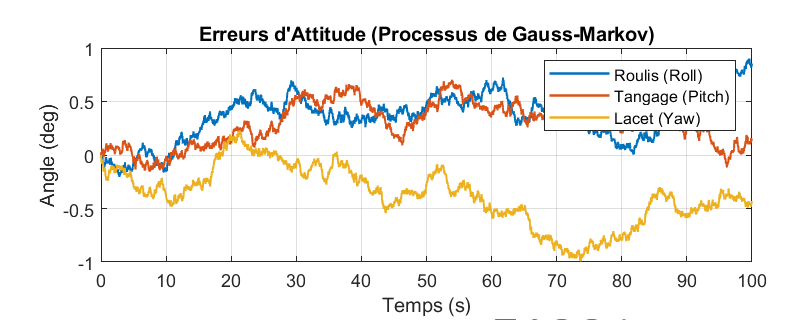
\includegraphics[width=0.7\linewidth]{src/rapport_complet/img/gauss-markov.png}
    \caption{Evolution des erreurs de phase }
    \label{fig:gauss-markov}
\end{figure}
\FloatBarrier
On définit la matrice de rotation correspondante $\mathbf{R}(\phi, \theta, \psi)$ est donnée par :

\begin{equation}
    \mathbf{R} = 
    \begin{bmatrix}
    \cos\psi \cos\theta & \cos\psi \sin\theta \sin\phi - \sin\psi \cos\phi & \cos\psi \sin\theta \cos\phi + \sin\psi \sin\phi \\
    \sin\psi \cos\theta & \sin\psi \sin\theta \sin\phi + \cos\psi \cos\phi & \sin\psi \sin\theta \cos\phi - \cos\psi \sin\phi \\
    -\sin\theta & \cos\theta \sin\phi & \cos\theta \cos\phi
    \end{bmatrix}
\end{equation}

On définit aussi le bras de levier $L$ et le vecteur de visée unitaire $u_{local}$. Le déplacement du centre de phase dû à la rotation du bras de levier à l'instant $k$, par rapport à sa position nominale, est exprimé par le vecteur de translation résiduel :
\begin{equation}
    \Delta \mathbf{L}_k = \mathbf{R}_k \mathbf{L} - \mathbf{L}
\end{equation}

La variation de distance radiale $\Delta R_k$ (déplacement projeté sur la ligne de visée) est alors obtenue par le produit scalaire :
\begin{equation}
    \Delta R_k = \mathbf{u}_{local} \cdot \Delta \mathbf{L}_k
\end{equation}

Enfin, pour un système radar fonctionnant à la longueur d'onde $\lambda$, l'erreur de phase $\Delta \Phi_k$ résultant de ce déplacement (en considérant le trajet aller-retour) est calculée par :
\begin{equation}
    \Delta \Phi_k = \frac{4\pi}{\lambda} \Delta R_k
\end{equation}
On obtient alors une série d'erreur de phase que l'on applique dans le domaine de l'historique de phase de l'image (signaux après compression en distance). 

\subparagraph{Mise en place de la scène}

Par la suite, il est nécessaire de se concentrer sur la mise en place de la scène. Notamment sur les cibles et la modélisation du bruit. 

La première itération de notre simulateur a défini les cibles en tant que points brillants parfaits avec une SER personnalisable. Bien que ces cibles soient peu réalistes dans notre contexte, elles permettent de valider la formation d'image en un point tout en observant les effets de bord amenés par la focalisation. 

Il aurait été intéressant d'ajouter d'autres types de scènes afin de caractériser plus précisément le simulateur et les algorithmes utilisés. Cependant, cela transformerait le projet en la réalisation unique d'un simulateur ce qui est complètement différent de l'objectif de SAR'DINE.

Par la suite, nous nous sommes intéressés à la modélisation du fouillis présent dans les images SAR. Afin de rester dans la philosophie simpliste de ce simulateur, nous avons cherché une modélisation simple mais efficace. La solution retenue est la simulation du sol comme une infinité de diffuseurs aléatoires. Cette représentation consiste à ajouter un bruit gaussien complexe aux données brutes issues du simulateur. Nous avons ici considéré que les antennes verrait le sol de la même manière et donc le déphasage appliqué est le même pour les deux antennes. 

Dans la même philosophie, nous avons fait le choix de ne pas modéliser le bruit thermique. En effet, il se serait limité à l'addition d'un bruit gaussien au données brutes ce qui est similaire au bruit de fouillis déjà simulé. 

\subsubsection{Résultats de simulation}\label{subsubsec:resultats_simu}

Les choix effectués dans la réalisation du simulateur sont maintenant expliqués et détaillés, il faut dorénavant analyser les résultats de ce dernier et explorer les paramétrages possibles afin de s'adapter au mieux au contexte de SAR'DINE.

Avant toute chose, il est important de définir les paramètres initiaux du simulateur. A noter que le paramètre qui changera entre deux simulations sera précisé dans leurs interprétations.
\FloatBarrier
\begin{table}[h!]
\centering
\begin{tabularx}{0.6\textwidth}{|l|X|}
\hline
\textbf{Paramètre}          & \textbf{Valeur} \\ \hline
$f_c$                       & $24.125~GHz$      \\ \hline
$B$                         & $250~MHz$         \\ \hline
$f_{ech_{ADC}}$             & $250~kHz$         \\ \hline
$T_{pulse}$                 & $10~ms$           \\ \hline
Gain                        & $13~dBi$          \\ \hline
$\theta_{el}$               & $12\degree$          \\ \hline
$\theta_{az}$               & $30\degree$          \\ \hline
$Ant_{spacing}$             & $12.7~mm$         \\ \hline
$v_{az}$                    & $0.05~m.s^{-1}$        \\ \hline
$d_{az}$                    & $2~m$             \\ \hline
$PRF$                       & $100$             \\ \hline
Cibles                      & $\bullet$ Cible 1 : $d=30 m$, $SER = 26 dBm^2$ \newline $\bullet$ Cible 2 : $d=50 m$, $SER = 26 dBm^2$ \\ \hline
Variance clutter            & $0$               \\ \hline
Erreurs d'Attitude          & Pas d'erreurs d'attitude au démarrage. \\ \hline
\end{tabularx}
\caption{Paramètres initiaux de simulation}
\label{tab:param_simu_init}
\end{table}
\FloatBarrier

Ci-dessous, on peut observer les résultats de simulation issus des paramètres initiaux. Comme on le remarque dans les deux graphiques inférieurs de la figure, les deux cibles sont facilement identifiables grâce à la présence des deux pics. De la même manière, on remarque l'absence de tout bruit lié au clutter ou aux erreurs de trajectoires. Par ailleurs, l'amplitude de la seconde cible est plus faible que celle de la première malgré une SER identique, ce qui valide la logique de simulation. 

\FloatBarrier

\begin{figure}[h!]
    \centering
    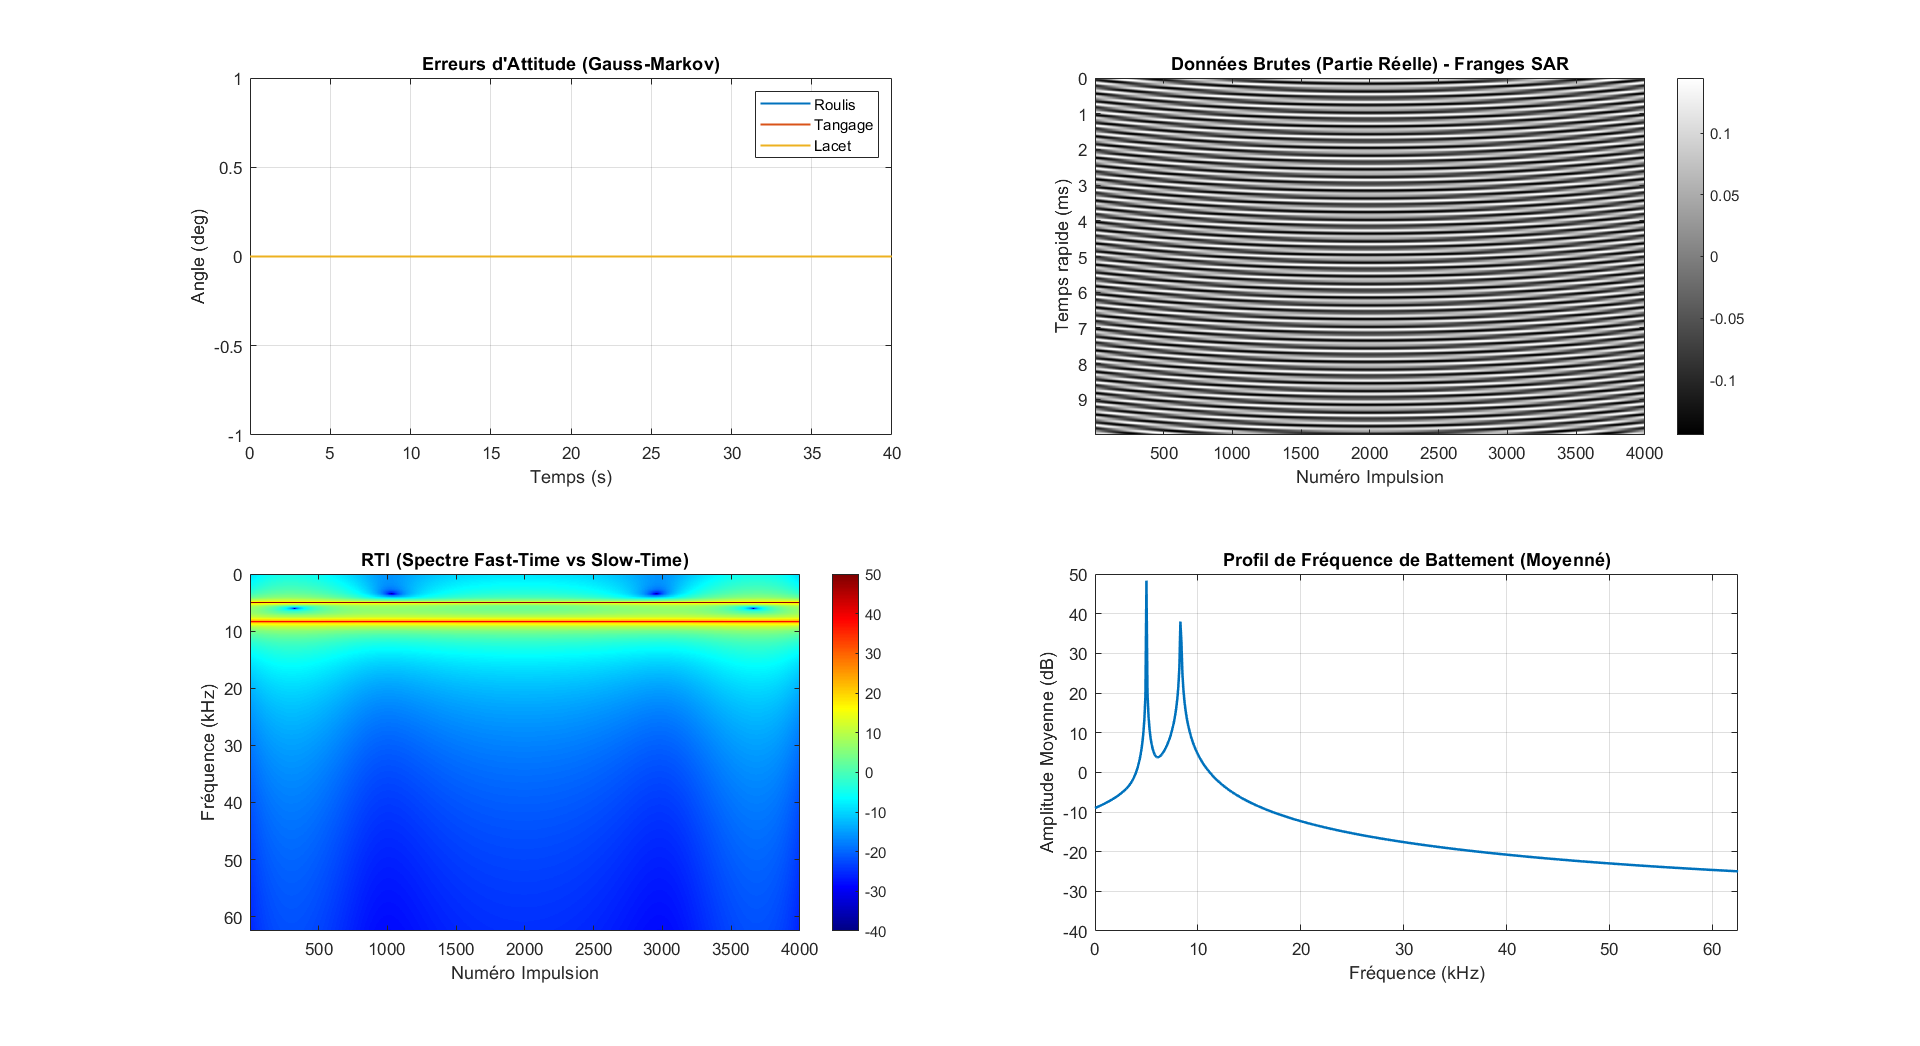
\includegraphics[width=0.8\linewidth]{src/rapport_complet/img/simu_2cibles_init.png}
    \caption{Résultats de simulation initiaux}
    \label{fig:resultat_simu_init}
\end{figure}

\FloatBarrier

Par la suite, nous allons mettre en place la simulation du clutter afin d'en observer les résultats. Ci-dessous se trouve les résultats de simulations avec une variance de clutter à $10^{-6}$. On observe l'apparition d'un fouillis sur le spectre temps rapide temps lent et ce dernier n'est pas visible sur le profil de fréquences de battement moyenné car la moyenne du clutter ajouté est nulle.

\FloatBarrier
\begin{figure}[h!]
    \centering
    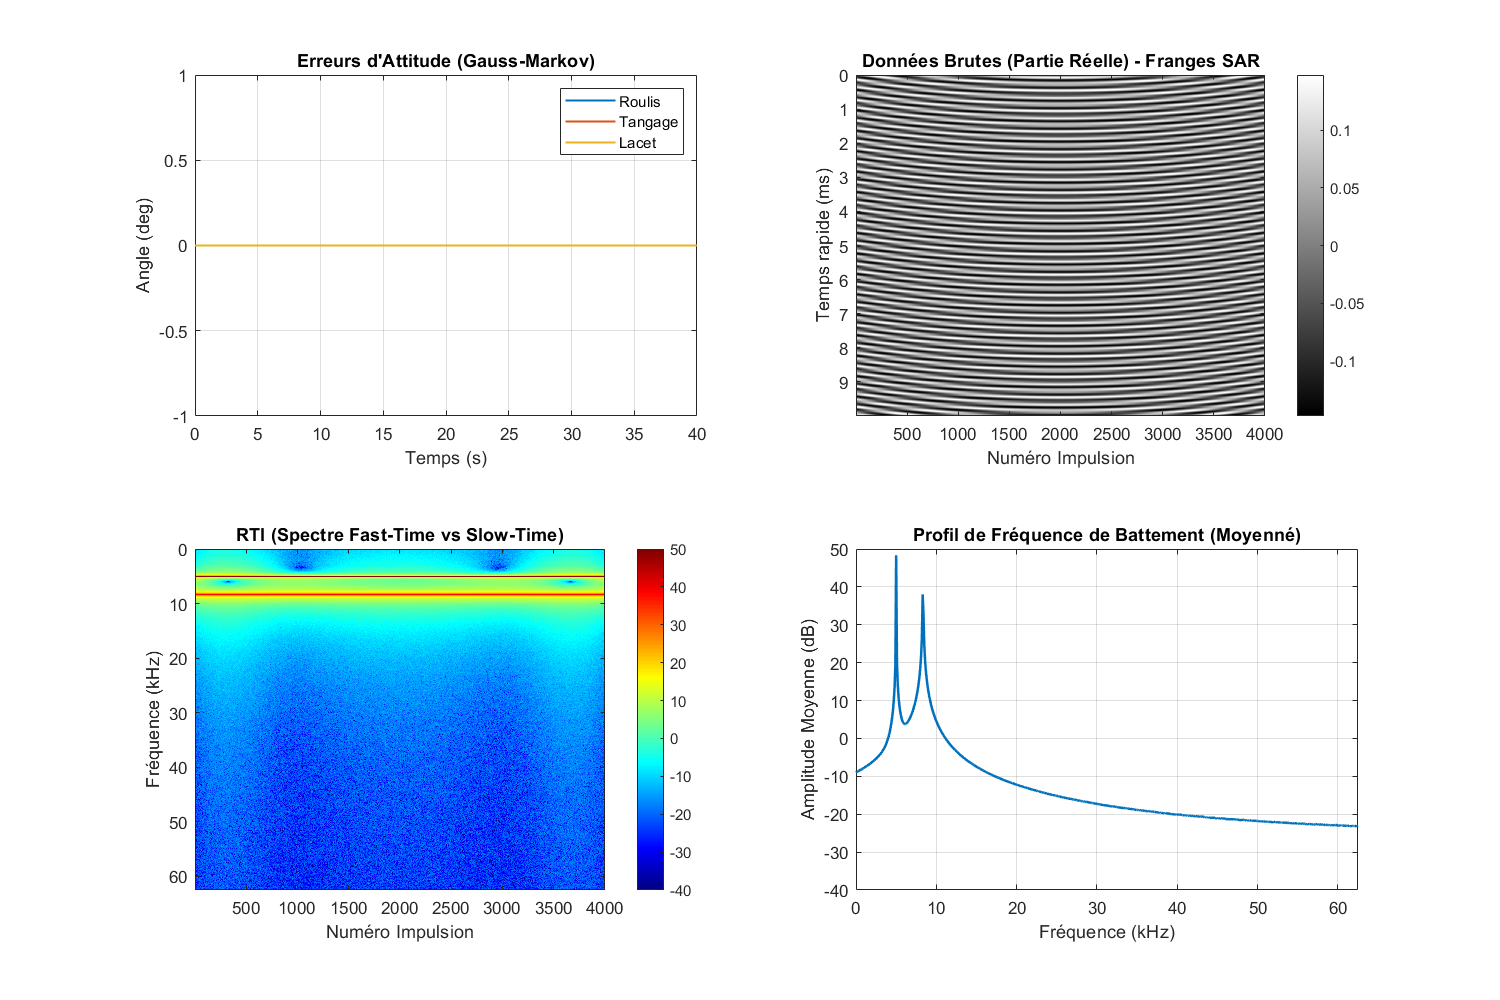
\includegraphics[width=0.8\linewidth]{src/rapport_complet/img/simu_2cibles_clutter-6.png}
    \caption{Résultats de simulation avec un clutter de variance $10^{-6}$}
    \label{fig:resultat_simu_clutter_-6}
\end{figure}
\FloatBarrier

On cherche maintenant à valider la simulation des erreurs de trajectoire détaillées dans le paragraphe \ref{subpar:erreurs_attitude}. Pour cela on lance une simulation en limitant le roulis, le tangage et le lacet à une erreur de 5\textdegree. On obtient alors le résultat présent dans la figure ci-dessous. On remarque que l'erreur se répercute sur le profil moyenné et sur le spectre range azimut. Cela s'explique car les erreurs d'attitudes désaxe l'antenne par rapport aux cibles qui récupère donc moins d'énergie.

\FloatBarrier
\begin{figure}[h!]
    \centering
    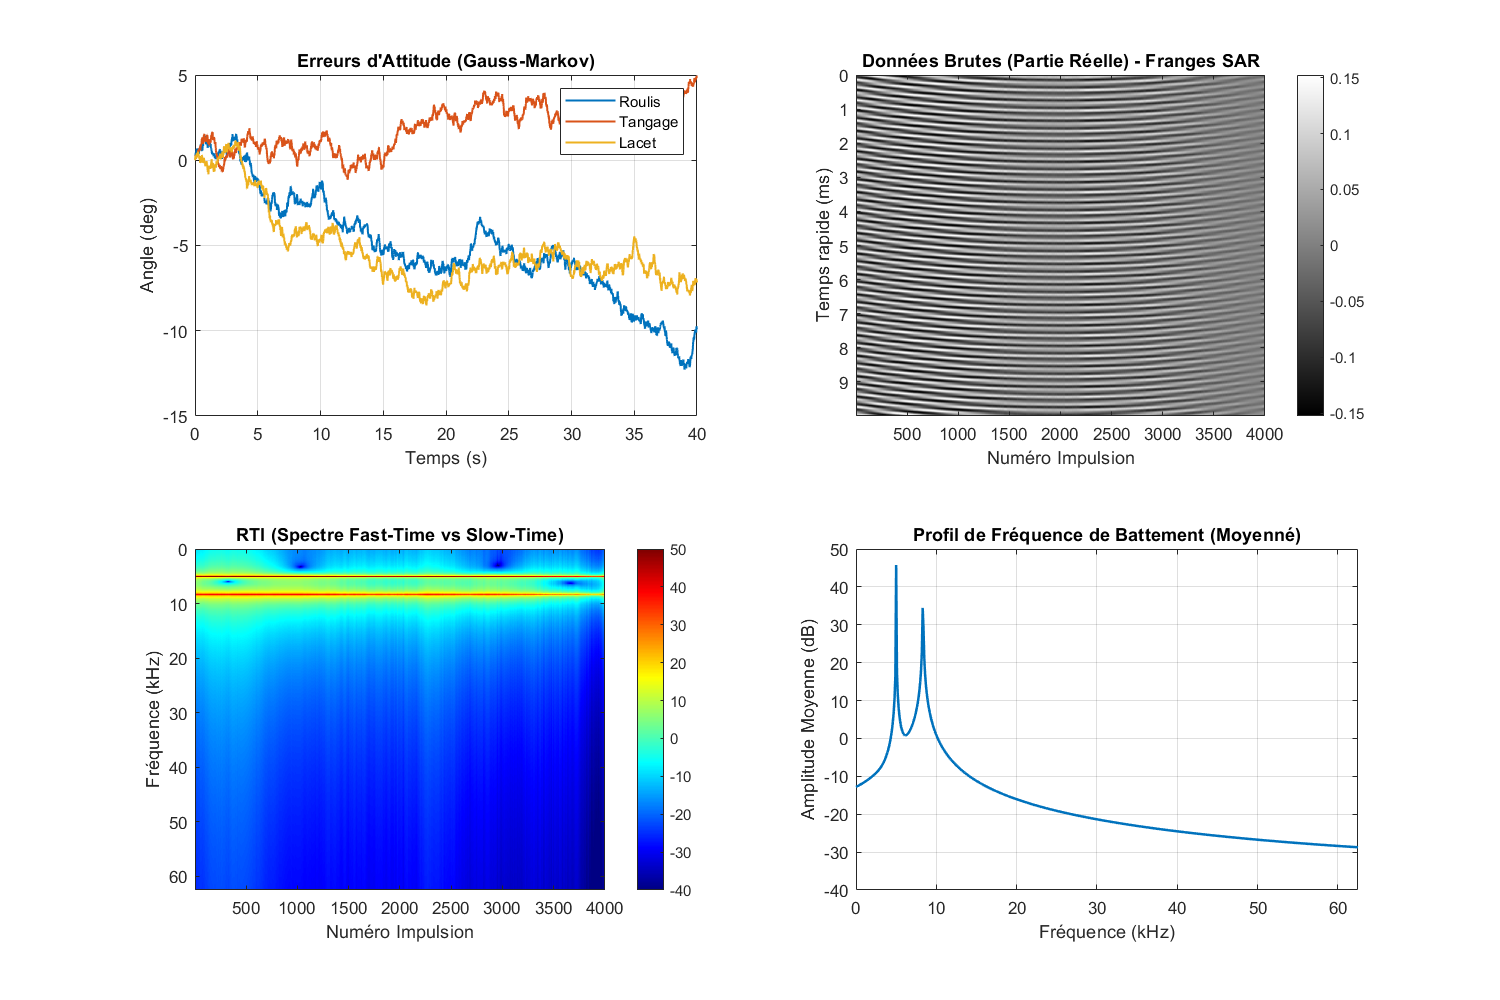
\includegraphics[width=0.8\linewidth]{src/rapport_complet/img/simu_2cibles_motion_5.png}
    \caption{Résultats de simulation avec erreurs d'attitude}
    \label{fig:resultat_simu_motion_5}
\end{figure}
\FloatBarrier

Le cas le plus proche de la réalité consistera à combiner à la fois des erreurs d'attitudes et du clutter. Ainsi, on observe sur la capture suivante que les deux erreurs peuvent être combinées dans le simulateur. 

\FloatBarrier
\begin{figure}[h!]
    \centering
    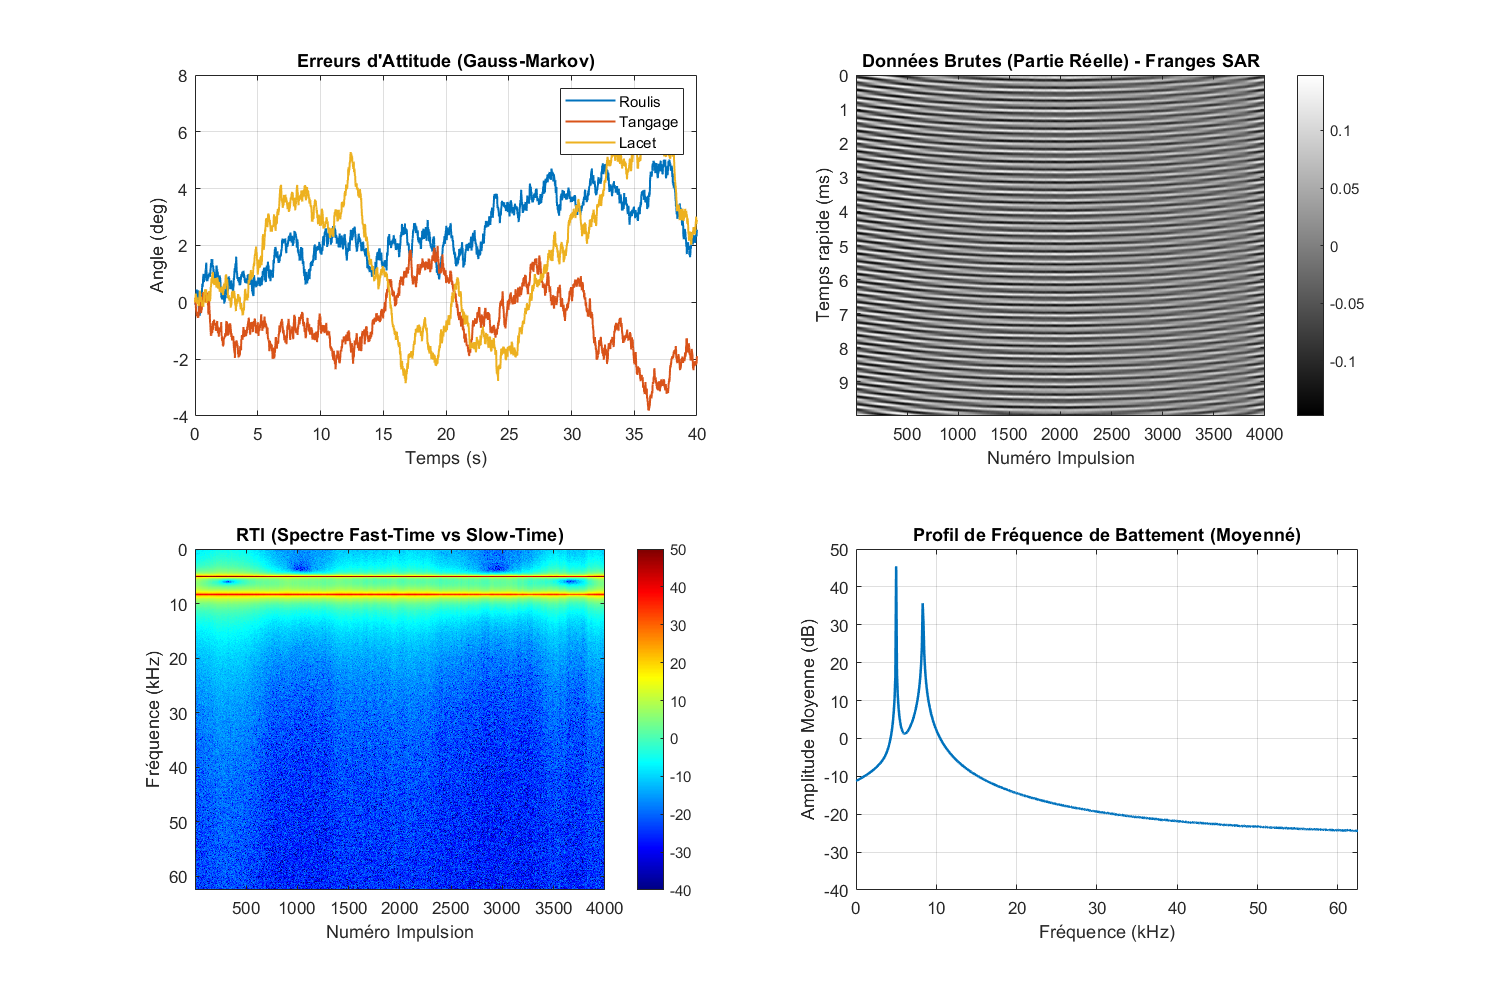
\includegraphics[width=0.8\linewidth]{src/rapport_complet/img/simu_2cibles_clutter-6_motion_5.png}
    \caption{Résultats de simulation avec clutter et erreurs d'attitude}
    \label{fig:resultat_simu_clutter_motion_5}
\end{figure}
\FloatBarrier

Ces résultats valident le fonctionnement du simulateur et sa capacité à adapter les conditions de simulation au plus proche de nos expérimentations. La simulation des erreurs d'attitude et du clutter permet d'avoir une scène plutôt réaliste ce qui est suffisant pour valider la bonne implantation de nos algorithmes de traitement.

% Config : 

% {
%   "radar": {
%     "description": "RFBeam K-MC4 Twin",
%     "fc": 24.125e9,
%     "bandwidth": 250e6,
%     "tx_power_dbm": 20,
%     "noise_figure_db": 12,
%     "adc_sample_rate": 250e3,
%     "adc_bits": 12
%   },
%   "modulation": {
%     "type": "triangular",
%     "sweep_time": 10e-3,
%     "start_frequency": 24.0e9,
%     "slope_linearity_error": 0.0
%   },
%   "antenna": {
%     "gain_dbi": 13,
%     "beamwidth_azimuth_deg": 30,
%     "beamwidth_elevation_deg": 12,
%     "rx_spacing_mm": 13.7,
%     "sidelobe_level_db": -20
%   },
%   "platform": {
%     "velocity_mps": 0.05,
%     "track_length_m": 2.0,
%     "start_position": [0.0, 0.0, 0.0],
%     "prf": 100
%   },
%   "scene": {
%     "targets": [
%       {
%         "id": 1,
%         "pos": [1, 40.0, 0],
%         "rcs": 26.0,
%         "description": "Cible Principale"
%       },
%       {
%         "id": 2,
%         "pos": [1, 50.0, 0],
%         "rcs": 26.0,
%         "description": "Cible Secondaire"
%       }
%     ],
%     "clutter_power": 1e-6
%   },
%   "motion": {
%     "enabled": true,
%     "tau_corr": 70,
%     "std_roll_deg": 0.5,
%     "std_pitch_deg": 0.5,
%     "std_yaw_deg": 0.5
%   }
% }
